% Name: Circular buffer
% Description: An eight-slot ring buffer holding four values, with the read pointer at the oldest value and the write pointer at the next free slot, wrapping round from slot 7 to slot 0.
% Tags: circular buffer, ring buffer, queue, data structures

\usetikzlibrary{arrows.meta}

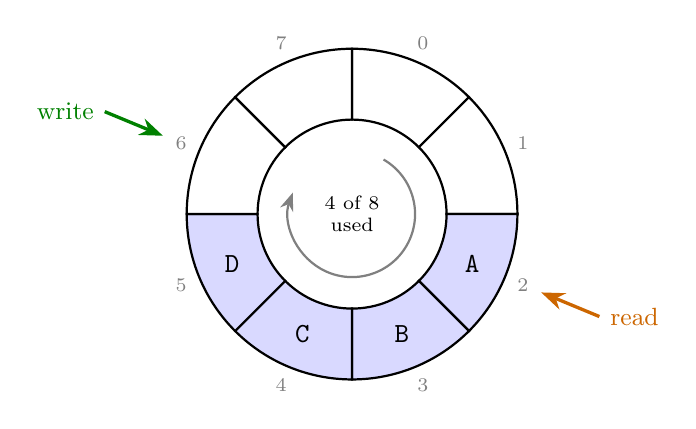
\begin{tikzpicture}[>={Stealth}, thick, every node/.style={font=\small}]
  % Slot k spans the angles 90 - 45k to 45 - 45k, so the slots run clockwise from the top
  \foreach \k/\v in {0/, 1/, 2/A, 3/B, 4/C, 5/D, 6/, 7/} {
    \pgfmathsetmacro\a{90 - 45*\k}
    \ifx\v\empty \def\f{white}\else \def\f{blue!15}\fi
    \draw[fill=\f] (\a:1.2) arc (\a:\a-45:1.2) -- (\a-45:2.1) arc (\a-45:\a:2.1) -- cycle;
    \node[font=\ttfamily] at (\a-22.5:1.65) {\v};
    \node[font=\scriptsize, gray] at (\a-22.5:2.35) {\k};
  }
  % Read at slot 2 (centre angle -22.5°), write at slot 6 (centre angle 157.5°)
  \draw[<-, orange!80!black, very thick] (-22.5:2.6) -- (-22.5:3.4) node[right] {read};
  \draw[<-, green!50!black, very thick] (157.5:2.6) -- (157.5:3.4) node[left] {write};
  \draw[->, gray] (60:0.8) arc (60:-200:0.8);
  \node[align=center, font=\scriptsize] at (0,0) {4 of 8\\used};
\end{tikzpicture}
